\documentclass[10pt,a4paper,twoside,openany]{article}

% Packages.
% \usepackage[options]{names,comma,separated}
\usepackage[T2A]{fontenc}
\usepackage[utf8]{inputenc}
\usepackage[bulgarian]{babel}

% Fonts listing. Exactly one must be selected.
% List all fonts with "locate /t2a | grep 'texlive/texmf-dist/tex/latex/.*\.fd$'".
% \usepackage{antt}      % Doesn't work.
% \usepackage{cantarell}
% \usepackage{cm-lgc}    % Doesn't work.
% \usepackage{comfortaa}
% \usepackage{cyrillic}  % Doesn't work.
% \usepackage{droid}
\usepackage{iwona}
% \usepackage{kurier}
% \usepackage{opensans}

\usepackage[pdftex]{graphicx}
\usepackage[table]{xcolor}     % For coloured rows within tables.
\usepackage{fullpage}          % Set left and right margin to 1 inch - much less than the default.
\usepackage{multicol}

% Macros, declared in separate headers.
% This file declares a template formagic skill desription through examples
% with specific difficulty values.

% Here is an example on how to use it:
%\begin{document}
%\spell{Small Heading}{example; example 2}{}{}{example 3}{}{}{}
%\end{document}

\usepackage{xparse}
\usepackage{ifmtarg}
\usepackage[T2A]{fontenc}
\usepackage[utf8]{inputenc}

\ExplSyntaxOn
\makeatletter
\newcommand{\spell}[8]{
    \par\noindent\textbf{#1}
    \par\noindent\underline{0\ ниво}
    \@ifmtarg{#2}{\par\vspace{\topsep}}{\list_examples:n{#2}}
    \par\noindent\underline{1\ ниво}
    \@ifmtarg{#3}{\par\vspace{\topsep}}{\list_examples:n{#3}}
    \par\noindent\underline{2\ ниво}
    \@ifmtarg{#4}{\par\vspace{\topsep}}{\list_examples:n{#4}}
    \par\noindent\underline{3\ ниво}
    \@ifmtarg{#5}{\par\vspace{\topsep}}{\list_examples:n{#5}}
    \par\noindent\underline{4\ ниво}
    \@ifmtarg{#6}{\par\vspace{\topsep}}{\list_examples:n{#6}}
    \par\noindent\underline{5\ ниво}
    \@ifmtarg{#7}{\par\vspace{\topsep}}{\list_examples:n{#7}}
    \par\noindent\underline{6\ ниво}
    \@ifmtarg{#8}{\par\vspace{\topsep}}{\list_examples:n{#8}}
}
\makeatother

\cs_new:Npn \list_examples:n #1{
    \seq_set_split:Nnn \splitted_seq{;}{#1}
    \begin{itemize}
        \seq_map_inline:Nn \splitted_seq{
            \item ##1
        }
    \end{itemize}
}
\ExplSyntaxOff

% This file declares a template for player races. Here is an example on how to use it:
%\begin{document}
%\race{Race name}{Point price}{}{}{example 3}{}{}{}
%\end{document}

\usepackage{xparse}
\usepackage{ifmtarg}
\usepackage[T2A]{fontenc}
\usepackage[utf8]{inputenc}

\ExplSyntaxOn
\makeatletter
\newcommand{\race}[8]{
    \par\noindent\textbf{#1}
    \par\noindent{Цена:\ #2} \\
                             \\
    Точки:
    \par\noindent{Сила:\ #3}
    \par\noindent{Ловкост:\ #4}
    \par\noindent{Ум:\ #5}
    \par\noindent{Харизма:\ #6}
                             \\
    Качества:                \\
    \@ifmtarg{#7}{\par\vspace{\topsep}}{\race_template_perks{#7}}
                             
    Расови умения:
    \@ifmtarg{#8}{\par\vspace{\topsep}}{\race_template_skills{#8}}
}
\makeatother

\cs_new:Npn \race_template_perks #1{
    \seq_set_split:Nnn \splitted_seq{;}{#1}
    \begin{itemize}
        \seq_map_inline:Nn \splitted_seq{
            \item ##1
        }
    \end{itemize}
}

\cs_new:Npn \race_template_skills #1{
    \seq_set_split:Nnn \splitted_seq{;}{#1}
    \begin{itemize}
        \seq_map_inline:Nn \splitted_seq{
            \item ##1
        }
    \end{itemize}
}
\ExplSyntaxOff


% Commands.
% \newcommand{name}[num]{definition}
\newcommand{\standout}[1]{\textbf #1}  % Anyone, who has read the rules, can skim through these sections for important information.

% Environments.
% \newenvironment{name}[num]{before}{after}
\newenvironment{shortstory}{\itshape}{}  % Fluff material, to get the reader in the mood for the incoming section.

\newcommand{\HRule}{\rule{\linewidth}{0.5mm}}  % Horizontal line.
\newcommand{\firstletter}{}  % Old book style huge, gorgeous first letter of the chapter.
\newcommand{\mychapter}{}  % A subsection title with an optional accompaning image.
\newcommand{\smallrules}{}  % Under a small heading, list consicely several unrelated rules (paragraphs).
% \newcommand{\alternateTableRowColor}{{\rowcolors}{1}{white}{lightgray}}  TODO: how to make this work?

% Document body.
\begin{document}
\begin{titlepage}
\begin{center}

% Upper part of the page. The '~' is needed because \\
% only works if a paragraph has stared.
\textsc{\Huge Елементарис}\\[1.5cm]
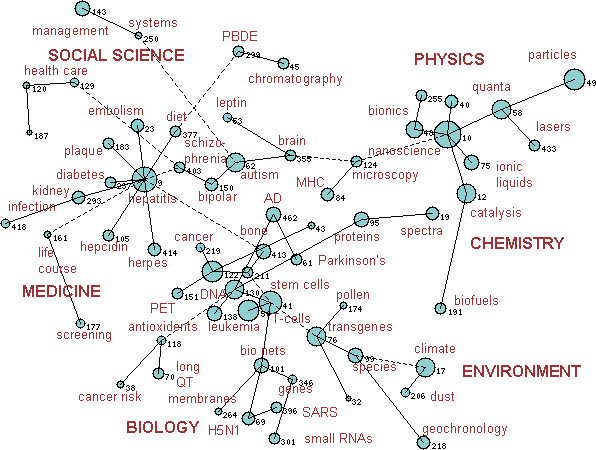
\includegraphics[width=0.85\textwidth]{../images/map-of-sciences}~
\\[1cm]

\vfill

% Bottom of the page.
\date{}

\end{center}
\end{titlepage}

\section{Игрови персонажи}
\emph{Ел'тлменел от селото Нлимна има резки чети за елф, и определено неестествен ръст на неговите метър и деведесет.
Олекотената ризница от еленски рога не приквива силните му ръце и крака, а копието и лъка допълват картината на ловец/войн, само тъмнозеленото ленено наметало остава.
Менел, както го наричат не-елфите навсякъде, е израстнал в гори, не умее да чете и е страшно глупав, когато става дума за светски дела.}

Героите на нашето приключение трябва да бъдат описани по прост, но съдържателен начин.
Това става с \textbf{дарби, показатели и умения}.

\subsection{Дарби}
Това са свойства на перонажа, с които той започва, и не се очаква да могат да бъдат променени някога.
Примери вкючват “Интуитивна ориентация в тъмното”, “Огнена кръв(раните не кървят, а веднага се затварят)”, “Слепота”.
Персонажът Нафарфорий/Пешо се създава с {\bfедно положително} == помагащо му качество.
Или до {\bfоще три}, като за всяко допълнително “хубаво” качество, си харесваме по едно “лошо”. Стига се цупи де, лошите качества са крайно забавни за разиграване!

\subsection{Показатели}
Разполагаш с \textbf{30 точки}, които да разпределиш по показателите. Те се променят рядко.
\begin{itemize}
\item {\bfСила} – телосложение, експлозивна сила, статична сила, умение да се концентрира силата на тялото, имунна система
\item {\bfЛовкост} – както пъргавина и гъвкавост на цялото тяло, скорост, така и прецизност във фините задачи
\item {\bfУм} – еродиция, памет, разсъдък, концентрация, наблюдателност, схватливост
\item {\bfХаризма} – увереност, емпатия, изразителност, излъчване
\end{itemize}

\subsection{Умения}
Начални точки и развиване  \\
С \textit{Ум * 5} разполагаш, за да разпределиш по умения.
Уменията, също така, се повишават с точки опит по време на игра.
\\
\\
Ниво на владеене  \\
Нивото на владеене на всяко умение се оценява по скала от 0 до 15, като 15 е специална стойност.
Всяко умение е базирано върху някой показател.
Половината от показателя (закръглено надолу) се добавя към ранговете на умението, когато то се ползва.
Повишаване на умение на повече рангове,  отколкото е показателят, струва по две точки за всеки ранг на умението.

\subsection{Носене}
\rowcolors{1}{white}{lightgray}
\begin{tabular}{l | l | l }
Максимален товар, кг & Придвижване, м            & Наказание  \\
Сила                 & Сила + Ловкост + Ловкост  & -0         \\
Сила * 2             & Сила + Ловкост            & -0         \\
Сила * 5             & Сила                      & -5
\end{tabular}


\subsection{Предмети}
Героите започват с един среден, три евтини и колкото си пожелаят много евтини предмети.
Прогресията е много скъп(замък) - скъп(имение) - среден(двуръчен меч) - евтин(меч) - много евтин(щит, брадва).

\section{Бойна система}
\emph{Копитата тракат, капрата проскърцва.
Ръми втори ден вече и макар промазаната качулка да пази лицето ми, ботушите ми са пълни с вода и джвакат.
Сют е кочияш на работа и пияница в другото време, вече от ден не сме си казвали нищо, нека си дърпа юздите.
\\
В гората напред край пътя – движение.
\\
“СПРИ!” викам.
Фургонът спира, конете цвилят.
Две къси копия прелитат, убиват единия кон.
Крадците връхлитат.
Хващам щита от куката и скачам, халчестата ризница дрънчи, вадя меча.
Вече замахва нож, устремявам щита към главата му и сека към коленете.
Удрям и го повалям, втори ми е странично и опитва да забоде ножа в ребрата ми, но ризницата пази.
Убивам го. От капрата връхлита секирата, отсяква главата на Сют.}

\vspace{5mm} \indent
От бойната система се очаква да е както проста и лесна, непречеща на разказването на историята, така и детайлна и категорична, позволяваща вглъбяване в динамиката на онези кратки моменти, в които страшно смелият ни герой е с единия крак в гроба.
В случай на ръкопашен бой се разглеждат отрязъци от по няколко такта на сърцето.
За такова време е достатъчно да замахнеш по арка с голямо оръжие, да нанесеш няколко удара с дръжка на пистолет или рапира, да извадиш стрела от колчана.
За престрелки се разглеждат отрязъци от порядъка на сто такта на сърцето.
Това отразява търсене на укритие, презареждане на арбалет или побиване на стрели в земята за лък, дебнене дупка в прикриващия огън при огнестрелни оръжия.
Действието се случва на най фината/бързата скала, присъстваща на бойното поле.
Например, когато тичащата пехота е на разстояние 300 метра от срелците с дълъг лък, играем по гранулярността за престрелки.
Бронираната милиция изминава разстоянието, стрелците правят 6 залпа на регулярни разстояние във времето.
След това настава клане и играем по гранулярността за меле.
Впрочем и двете групи са сега изморени, тъй каот са прекарали цял дълъг хот в интензивно натоварване, и търпят наказание от -5.

\subsection{Тактове време}
\subsection{Ръкопашни дистанции}
\begin{enumerate}
\item{директна (борба)}
\item{близка (нож, невъоръжен, къс меч)}
\item{средна (меч 80см, повечето оръжия за една ръка)}
\item{дълга (дълъг меч, копие, двуръчен меч)}
\item{отдалечена (пика)}
\item{извън ръкопашен обхват (стрелящи неща)}
\end{enumerate}
Инициатива за първия удар има този с по-дълго оръжие (очевидно).
Извън оптималната си дистанция, оръжията са на -5 атака и половин щети.
Придвижване между дистанции се извършва след успешно хвърляне (независимо нападение или защита).
Придвижването е или една категория в произволна посока или произволен брой категории, без да се преминава през заплашвани от някой враг дистанции. 

Пример:
\emph{Пешо, с копие и нож, напада Жоро, с меч.
Пешо връхлита и напада с копието.
Хвърля боравене + d6* < боравене на Жоро.
Жоро е отбягнал атаката и може да промени дистанцията.
Пешо заплашва дълга (копие една ръка) и близка(нож)
Жоро може да избере близка, средна, дълга, отдалечена или да избяга.
}

\subsection{Стрелба}
Защитата на движеща се цел се равнява на нейната ловкост.

\subsection{Оръжия}
Една характеристика на оръжията е обсегът от Сила, за който са ефективни
Ако персонажът има по-малко от минималната сила, разликата става наказание върху боравенето с това оръжие.
От друга страна, Сила, по-висока от максималната, не допринася за по-високи щети.
Друга характеристика са щетите на оръжието. Условно наричаме “ниски” щети от малки оръжия за една ръка, “средни” - тези на по-големите едноръчни оръжия и “високи” тези на повечето двуръчни оръжия.
Самото оръжие може да има бонус или наказание върху щетите си, редом с качествата на оръжието.
Обсегът на оръжията има различен смисъл за ръкопашни и далечни оръжия.
При ръкопашните оръжия, това е оптималната дистанция.
На всички по-близки дистанции оръжието има наказание от -5 боравене и половин щети.
За далечни оръжия, обсегът е максималното разстрояние, на което лесно може да се улучи цел.
На по-голямо от това разстояние атаката е с -5 наказание, на по-голямо от два пъти това разстояние става -10 и на от три до четири пъти това разстояние е на -15.
Чести стойности за обсег са (Сила/2) – метателен нож, (Сила) – метателно копие, (Сила х 2) – лък .

Също така, оръжията могат да имат някои от следните свойства.
\begin{enumerate}
\item{повратливост (обикновено мечове; покрива всички по-близки дистанции от максимлната)}
\item{бронебойност I (чукове или леки клинове, като стрели и копия; намаля абсорбацията на половина)}
\item{бронебойност II (клиновидни, тежки остриета; намаля абсорбацията на $\frac1 4$)}
\item{трудно за вадене (не може да се извади от пробита проня по време на битка; не може да се извади от небронирана плът, ако зарът за щета е бил положителен; при вадене лечитеслтво с/у щетите; ако не успее се  нанасят още толкова щети, колкото първоначално)}
\item{поваляне (обикновено алебарди; наместо щети, атаката може да бъде обявена, че поваля опонента. Ако целта е конник в качествено бойно седло, -5 на атака)}
\item{обезоръжаване (обикновено меч или щит; при успешна защита има шанс оръжието на врага да е уловено в комплексния гард или шипове на "бос"a на щит)}
\end{enumerate}

\subsection{Брони}
Защитната стойност на броните се получава от това каква част от тялото е общо покрита.
Пазене:
\begin{itemize}
\item{Шлем за темето(селяшки, евентуално с периферия) 1}
\item{Шлем с открито лице(с набузници или кръст за носа и очите, каска) 2}
\item{Шлем със забрало(пълен шлем) 3}
\item{Яка (към пълен шлем или като отделен компонент) +1}

\item{Кираса/Бронежилетка 5}

\item{Паудрони (част от ризница с къси ръкави или като отделен компонент) +1}
\item{Налакътници (част от дълга ризница или отделен компонент) +1}
\item{Ръкавици +1}

\item{Сабатони (бронирани ботуши) +1}
\item{Грейвси (броня от коленото надолу по пищяла) +1}
\item{Набедреници(може да е пола, част от дълга ризница или отделен компонент) +1}
\end{itemize}

Общо максимум: 15

Здравина:
Кожена броня(слоеве памук/хартия/коприна/мека кожа, със зашити плочи варена кожа/хитинова коруба на негъвкавите части) 4
\begin{itemize}
\item{Халчеста броня, подплатена с гамбезон 6}
\item{Ламенарна броня, подплатена с гамбезон 9}
\item{Лята броня, подплатена с гамбезон(средновековен дизайн - субоптимална форма, субоптимална стомана, примитивно закаляване, подвижност в ставите се осигурява от халчести участъци) 12}
\item{Лята броня, подплатена с гамбезон(ренесансов дизайн - скосени повърхности, качествена стомана (high toughness core),  интелигентно закаляване на повърхностния слой(hardened shell), сложни механични стави) 15}
Теглата на копонентите клонят към една десета от произведенито на покритието и здравината си.
\end{itemize}

\subsection{Механика}
Нека си дойдем на думата.
Удар или група удари (едно ръкопашно действие) се групират в обща цел – нападение или защита.
Нападащият добавя d6* към боравенето си и сравнява с боравене на отбраняващият се, който се отбранява с всички средства налични – отбягва, парира.
Подробности:
\begin{itemize}
\item[-]{отбраняване само чрез отбягване носи наказание от -5, но добавя +5 на боравене при атаки срещу тази конкретна цел на следващия ход}
\item[-]{отбраняване от втори нападател търпи наказание от -5; от трети общо -10 и т.н.}
\end{itemize}

Ако нападателя има повече, съществени удари са достигнали целта.
Ако нападателя има повече от боравене на защитника + пазене на броните му, поне един удар е попаднал в небронирана област.

\subsection{Специални правила}
\begin{center}
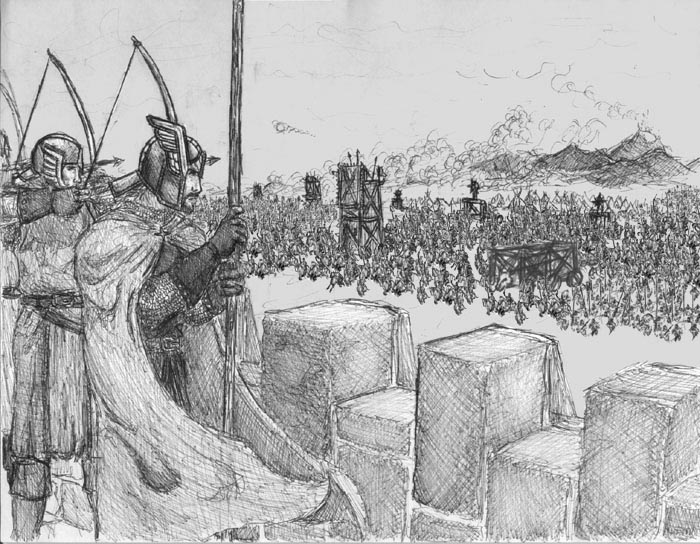
\includegraphics[width=0.75\textwidth]{../images/siege}~
\\[1cm]
\end{center}

\subsubsection{Кавалерия}

\subsubsection{Езда}
\begin{itemize}
\item[-]{нивото на ползване на умения от гърба на кон е ограничено до нивото на умението “езда”}
\item[-]{ръкопашни атаки от и по ездач на галопиращ кон са с двойни щети}
\item[-]{атаки от и по ездач на кон с късо оръжие търпят -5 атака}
\end{itemize}

\subsubsection{Две оръжия}
Едното оръжие се ползва за да нанесе щети на врага, нека наречем него първо.
Второто оръжие може да се ползва за създаване на откриване (което добавя половината боравене в това оръжие към боравенето с основното оръжие) или пък независимо, за пласиране на стопиращи удари (в който случай се ползва независимо, но с наказание -5 на атака).
Ако се атакува само с едното оръжие няма наказания, разбира се.

\subsubsection{Щит}
\begin{itemize}
\item[-]{Щитът е направен да е второ оръжие. Като такъв не търпи -5 когато се ползва за защита.}
\item[-]{пазене от стрели 0/6 (бъклър) през 2/6(кръгъл викингски) през 4/6(дълъг римски) до 6/6 (павис). Това когато активно се криеш от стрелите, разбира се.}
\item[-]{Дървените щитове имат здравина 15, а стоманените 30. Това обикновено няма значерние, но силни или бронебойни атаки може да преодолеят успешно блокиране.}
\end{itemize}

\subsection{Таблица щети}
Сила *1/2 *2/3 *1
1  d-3  d-3  d-2
2  d-3  d-2  d-1
3  d-2  d-1  d-1
4  d-2  d-1  d+1
5  d-1  d    d+2
6  d-1  d    d+3
7  d    d+1  2d
8  d+1  d+2  2d+1
9  d+1  2d-1 2d+2
10 d+2  2d   3d
11 d+2  2d   3d+1
12 2d-1 2d+1 3d+2
13 2d-1 2d+2 3d+3
14 2d   3d-1 4d
15 2d+1 3d   4d+1
16 2d+1 3d+1 4d+2
17 2d+2 3d+1 5d
18 2d+2 3d+2 5d+1
19 3d-1 4d-1 5d+2
20 3d-1 4d   5d+3
21 3d   4d   6d
22 3d+1 4d+1 6d+1
23 3d+1 4d+2 6d+2
24 3d+2 5d-1 7d
25 3d+2 6d   7d+1
26 4d-1 5d   7d+2
27 4d-1 5d+1 7d+3
28 4d   5d+2 8d
29 4d+1 6d-1 8d+1
30 4d+1 6d   8d+2

\chapter{Магия}
Хвърля се Умение + Ум / 2 срещу зададена от Разказвача трудност. При
неуспех, разликата се прилага като травма.

Магически кръгове могат да изричат заклинания синхронизирано. Трудността
на заклинанието се разпределя между магьосниците както те решат. След това
всеки хвърля срещу собственото парче трудност. Ако някой се провали,
изричанеот се проваля и всеки търпи съответните щети.

За всяко настоящо поддържано заклинание от същата школа магия, умението се
намаля с 5 точки временно.

\section{Заклинания}

\textbf{Жизнена енергия / Некромантия / Отвъд}
\begin{itemize*}
  \item{укротяване на звяр - 5}
  \item{усещане за немъртви - 5}
  \item{лекуване (умение + d6* ЖТ) - 5}
  \item{изтляване - съществото умира след месец  докато се поддържа магията - 10}
  \item{скелетен слуга - <умение + д6*> по показатели, следва вербални команди - 10}
  \item{убиване - <умение> с/у <сила на опонента> - 15}
  \item{възкресяване на тяло - 20}
  \item{възкресяване по спомен - 25}
  \item{възкресяване по описание - 30}
  \item{превръщане в лич - 30}
\end{itemize*}

\vspace{1cm}
\textbf{Гадание / Пророчество (в пространството и времето)}
\begin{itemize*}
  \item{усещане позицията на предмет след докосване, до няколко километра - 5}
  \item{усещане името на същество - 5}
  \item{виждане на далеч - 5}
  \item{светлина - 5}
  \item{живо оръжие (бoравенето става равно на умението гадаене) - 10}
  \item{уцелване отвъд прикритие (атака = умение) - 10}
  \item{виждане през стени - 10}
  \item{усещане на лъжи - 10}
  \item{виждане в тъмнина - 10}
  \item{посока към най-близкия град/път/река - 10}
  \item{предсказване на удари - +умение към боравене - 15}
\end{itemize*}


\vspace{1cm}
\textbf{Огън}
\begin{itemize*}
  \item{запалване на много свещи - 5}
  \item{запалване на дрехи - 5}
  \item{предпазване от жега - 5}
  \item{огнено копие - Щ = умение, високи, 10}
  \item{палене на колиба - 10}
  \item{запалване на човек - 10}
  \item{защита от огън - 10}
  \item{огнено кълбо - <умение> радиус - 15}
  \item{запалване на тълпа - 15}
  \item{защито от огън на тълпа, 15}
  \item{запалване на град - 20}
  \item{езеро от лава - 20}
  \item{защита от огън на град - 20}
\end{itemize*}

Бъдещи идеи:  \\
Вятър (Ум)        - мъгла, ниво 2 мълния щяти по Ум, високи.                                         \\
Форма (Ум)        - превръщане на предмети или същества в други, промяна на показатели и размери     \\
Отвъд (Ум)        - разговаряне с души, вдигане на мъртви.                                           \\
Създаване (Ум)    - храна и вода, предмети и създания.                                               \\
Миъл (Ум)         - отношение и спомени                                                              \\
Tелепортация (Ум) - пътуване в този и други светове, с товари                                        \\







\chapter{Раси}
%Метаправила:  \\
%Качествата струват съответно по 1 и -1 точка за положителни и отрицателни качества.  \\
%Правото на две расови умения на 5, без да е нужно да покриват изисквания, без точките да се плащат от (5 * Ум), струва една точка.  \\
%Човеците имат всикчи показатели 1 - 10.  \\
%За всеки 3 точки по максимуми над 10, расата струва още една точка.  \\
%За всеки 5 точки по минимуми, расата струва една точка по-малко.  \\
%\\
\begin{multicols}{2}
\race{Homo Sapiens}{0}
{Доплавали на Ендивал от юг преди 4 века и провъзгласили Каланор и обширната Луседум Терея.}
{1 - 10}{1 - 10}{1 - 10}{1 - 10}{няма}{няма}

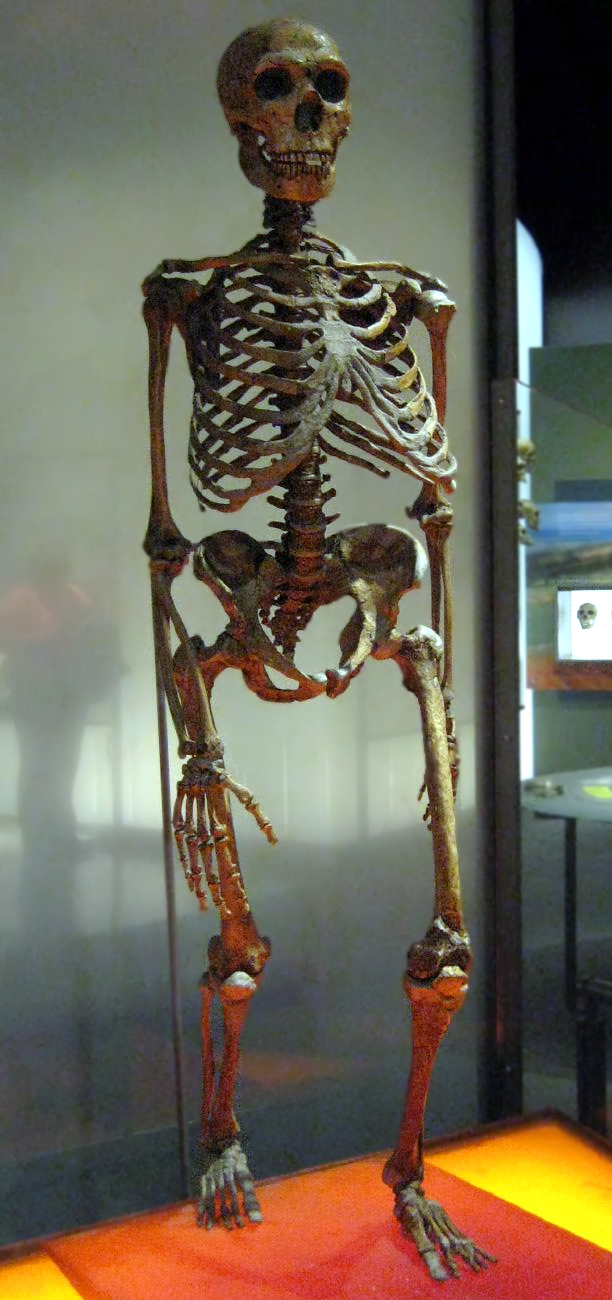
\includegraphics[height=0.25\textheight]{neanderthal1}
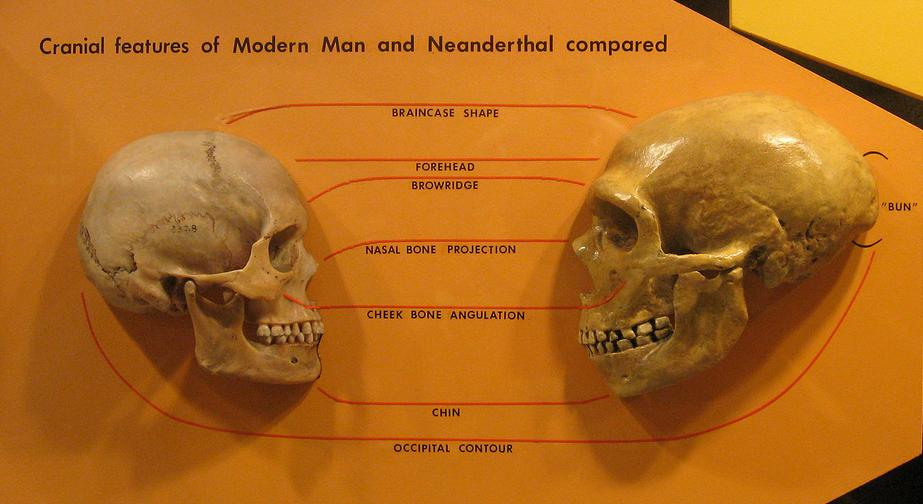
\includegraphics[height=0.25\textheight]{neanderthal2}
\race{Неандерталец}{1}
{}
{1 - 12}{1 - 11}{1 - 10}{1 - 10}
{няма}
{
Каменоделство(С)
Лов(Л)
Тичане(Л)
Копие(Л)
Промъкване(Л)
Билкарство(У)
}

\race{Джудже}{2}
{Местно население на Ендивал, което след пристигането на хората се разединява на три, а после на четири, кралства.}
{6-15}{1-8}{1-12}{1-8}{Виждане в тъмнина}
{
Джуджешки език(У);
Каменоделство(Л);
Боравене с брадва/чук(Л);
Металургия(У);
Ковачество(С)
}

\race{Елф}{4}
{Първите жители на Ендивал, сега са изтласкани до най-западните гори на континента.}
{1-8}{6-15}{1-15}{1-12}{Неспящ; Нестареещ}
{
Елфичеки език(У);
Лък(Л);
Катерене();
Магия - по избор(У);
Оцеляване в дивото(У)
}

\race{Върколак}{3}
{Създадени от Хазерот като по-съръшена раса от елфите.}
{6-16}{1-10}{1-10}{1-10}{Силна имунна система}
{
Оцеляване в дивото(У);
Вълчи език(У);
Човешки език(У);
Магия-огън(У);
Спринт(С)
}

\race{Здрачник}{4}
{Пришълци броени години преди човеците. Изтласкани да владеят горите от желязно дърво и търговията в Ендивал.}
{1-8}{1-15}{1-10}{6-16}{Изчезване в сянка}
{
Катерене(Л);
Оцеляване в дивото();
Търговия(Х);
Акробартика(Л);
Здрачничрски език(У)
}

\race{Немъртъв}{2}
{Когато немъртвите слуги станали често срещани, достатъчно от тях успяли да заменят връзката за управление от господаря си с връзка за управление към друг немъртъв.
Така те били способни да действат по собствена воля и да завладеят малко краство в северен Ендивал.}
{1-14}{1-9}{1-10}{1-4}
{
Усещане на живот (30 метра);
Телепатия;
Нестареещ;
Уязвими в ярко слънце (всчики хвърляния -10)
}
{
Магия-некромантия(У);
Поклонничество-Смърт(Х);
Строителство(У);
Тактика(У); %??
Език на немъртвите(У)
}

\race{Ниог}{5}
{Тези антропоморфни птици владеят сръчно телекинеза.
Живеят в технологични планински градове.
Са поколението на експедиция до Ендивал, която не успяла да се завърне.}
{1-6}{1-10}{1-14}{1-10}
{
Реене (може да планира по вятъра или да се издига от топли течения)
Отлитане (може да отлита и каца верикално)
Телекинеза (може да манипулира предмети до (Ум) метра със силата на една ръка и Ловкост 1)
Телекинетична сръчност (хаптична обратна връзка, както и фин контрол върху движенията)
}
{
Староендивалски език(У);
Астрономия(У);
Архитектура(У);
Употреба на обсадни оръжия(У);
Тaктика(У)
}

\race{Орк}{-2}
{Едри, раздразнителни и тъкмозелени на цвят.
Живеят в планински села и се препитават от лов и бандитлък.}
{1-16}{1-8}{1-6}{1-4}
{
Жажда за кръв %???
}
{
Език на гоблините(У);
Боравене с брадва(Л);
Оцеляване в дивото(У);
Строеж на лагер(У);
Проследяване в дивото(Л)
}

\race{Гоблин}{-3}
{Една от малкото раси, която успешно съжителства с орките.
Пристигнали заедно на Ендивал преди 12 века през подземен тунел.}
{1-6}{1-8}{1-8}{1-9}
{
Ранна старост
}
{
Език на гобилините(У);
Скриване от поглед(Л);
Капани(Л);
Плуване(С);
Катерене(Л)
}

\race{Драконит}{4}
{Човек с драконова кръв във вените си.
Драконитите живеят в малки, но строго регулирани племена, по склоновете на вулкани но и навсякъде, където е горещо.
Манюто им включва малки количества сяра и фосфор (няколко щипки на ден).}
{5-13}{1-10}{2-13}{1-10}
{
Неуязвимост от огън
Нестареещ
}
{
Език-драконски(У);
Магия-огън(У);
Магия-пазене(У);
Двуръчен меч(Л);
Древни легенди(У)
}

\end{multicols}

\section{Предмети}


\newcommand{\weapon}[8]
{
\begin{multicols}{2}
\noindent #2 \\
Необходима сила: #3  \\
Обсег: #4  \\
Щети: #5  \\
Свойства: #6  \\
Маса: #7  \\
Стойност: #8  \\
\includegraphics[width=0.2\textwidth]{../images/#1}~
\end{multicols}
}

\weapon{sword}{Меч}{5-12}{среден (0.9м)}{средни (//-2)}{повратливост}{1.1кг}{евтин}


\subsection{Валути}
Абстрактна валута: много евтиn, евтин, среден, скъп, много скъп; няма преобразувания.  \\
Луседом Терея: 100 имперски крони = 10 имперски рояла = 1 имперски соверен             \\
Каланор: 100 кралски крони = 10 кралси рояла = 1 кралски соверен                       \\
Сзал Тлея: 13 тъмни монети = 1 черна монета; 900 черни монети = 1 дълбока монета       \\
Креол: 1900 монети за храна = 1 монета за оръжие; 69 монети за оръжие = 1 монета за дом

\subsection{Надници}
Приходи за година. Стойностите в скобите не са ликвидни.
крепостен селянин
страж
ковач
майстор на лъкове
проститутка
лорд-робовладелец
войник
рицар
гробар

% Business / Population required per instance of business (called Support Value or SV)
\rowcolors{1}{white}{lightgray}
\begin{tabular}{p{3cm} | p{2cm}}
обущар      & 150   \\
кожар       & 250   \\
слугиня     & 250   \\
шивач       & 250   \\
бръснар     & 350   \\
бижутер     & 400   \\
таверна     & 400   \\
хлебар      & 500   \\
зидар       & 500   \\
дърводелец  & 550   \\
тъкач       & 600   \\

\end{tabular}

Chandlers     700
Mercers     700
Coopers     700
Bakers                   800
Watercarriers     850
Scabbardmakers   850
Wine-Sellers     900
Hatmakers     950
Saddlers     1,000
Chicken Butchers  1,000
Pursemakers     1,100
Butchers     1,200
Fishmongers     1,200
Beer-Sellers     1,400
Buckle Makers     1,400
Plasterers     1,400
Spice Merchants   1,400
Blacksmiths     1,500
Painters     1,500
Doctors                   1,700*
Roofers       1,800
Locksmiths     1,900
Bathers                   1,900
Ropemakers     1,900
Inns                   2,000
Tanners                   2,000
Copyists    2,000
Sculptors    2,000
Rugmakers    2,000
Harness-Makers  2,000
Bleachers    2,100
Hay Merchants    2,300
Cutlers                  2,300
Glovemakers   2,400
Woodcarvers   2,400
Woodsellers   2,400
Magic-Shops   2,800
Bookbinders   3,000
Illuminators   3,900
Booksellers   6,300
*These are licensed doctors. Total doctor SV is 350.

Some other figures: There will be one noble household per 200 population, one lawyer ("advocate") per 650, one clergyman per 40 and one priest per 25-30 clergy. Businesses not listed here will most likely have an SV from 5,000 to 25,000! The "Magic Shop" means a shop where wizards can purchase spell ingredients, scroll paper and the like, not a place to buy magic swords off the shelf. 
% The SV list was taken (mostly) from the tax list of Paris in 1292, and checked against other sources for accuracy.
% This list can be found in Life in a Medieval City by Joseph and Francis Geis (Harper and Row, 1981).
% This is a fine book by amateur historians, which includes some fascinating descriptions of medieval city life and layout.
% <quoted>

\subsection{Сгради}
\rowcolors{1}{white}{lightgray}
\begin{tabular}{p{3cm} | p{3cm} | p{3cm} | p{3cm} | p{3cm}}
мн. евтин & евтин                                   & среден                   & скъп                           & мн. скъп  \\
щит       & меч                                     & двуръчен меч             & имение                         & замък     \\
брадва    & халчеста къса ризница                   & боен кон                 & пълна броня пазаене 15 здр. 15 &           \\
куче      & кован нагръдник                         & качествена кираса и пола & качествена пълна броня         &           \\
колиба    & къща в малък град или село              & къща в голям град        & централна къща в столицата                 \\
          & магаре С30                              & боен кон                 &
\end{tabular}

\subsection{Оръжия}
\begin{tabular}{p{2cm} | p{2cm} | p{2cm} | p{2cm} | p{2cm} | p{2cm} | p{2cm}}
Наименование          & Необходима Сила      & Обсег      & Щети (Щм, Щс, Щт)       & Свойства       & Маса  & Стойност     \\
% Едноръчни оръжия.
Нож                   & 3-9                  & близък     & ниски (//-2)      & -              & 0.2кг & много евтин  \\
Брадвичка             & 5-12                 & среден     & средни, (-4//-2)  & бронебойност   & 1кг   & много евтин  \\
атаки: средна средни -4//-2 близка -4//-2
Къс меч               & 4-10                 & близък     & средни, (/-2/-4)  & повратливост   & 1кг   & евтин        \\
атаки: 
Меч 80см              & 5-12                 & среден     & средни, (//-2)    & повратливост   & 1кг   & евтин        \\
атаки: среден /-2/-4 близък //-2
Рапира                & 5-12                 & далечен    & средни, (+2/-2/0) &                & 1кг   & среден       \\

% Двуръчни оръжия.
Пика (две ръце)       & 4-11                 & отдалечен  & средни     & -              & 3кг   & евтин        \\
Дълга бойна брадва    & 5-12                 & далечен    & високи     & бронебойност   & 2кг   & евтин        \\

име, необходима сила!, дължина, щети, свойства, маса, стойност, изображение
Меч                   & 5-12                 & 0.9м     & средни (//-2)    & повратливост   & 1.1кг   & среден       \\
\begin{center}
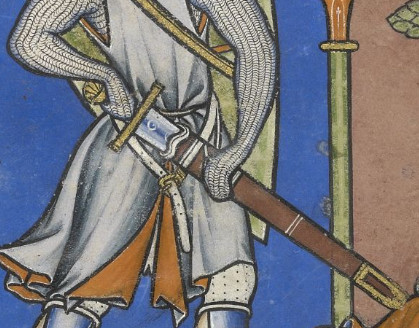
\includegraphics[width=0.75\textwidth]{../images/sword}~
\\[1cm]
\end{center}

Дълъг меч             & 5-12                 &  1.3м     & високи (//-2)    & повратливост   & 1.5кг   & среден       \\
\begin{center}
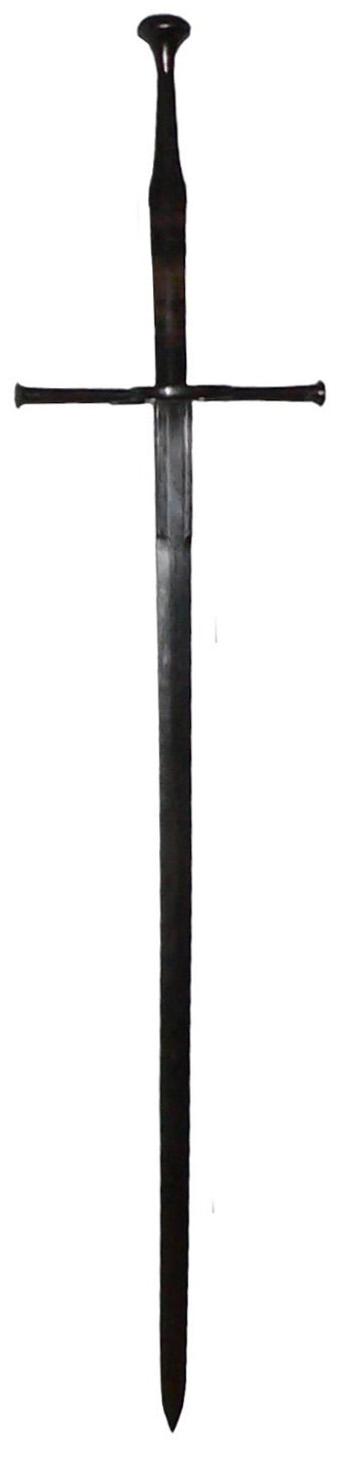
\includegraphics[width=0.75\textwidth]{../images/longsword}~
\\[1cm]
\end{center}

Цвайхендер            & 8-15                 &  2.1м     & високи (//-2)    & -              & 3кг   & среден       \\
\begin{center}
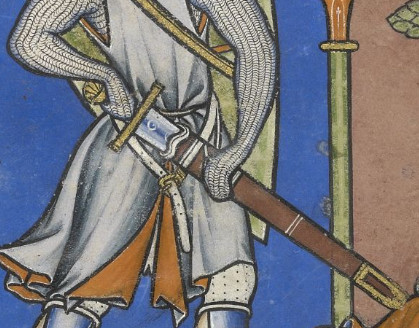
\includegraphics[width=0.75\textwidth]{../images/sword}~
\\[1cm]
\end{center}

Фалкс                 & 5-12                 & 1.5м   & високи (//-2)    & +2 на всички хвърляния срещу щитове   & 1.5кг   & евтин       \\
\begin{center}
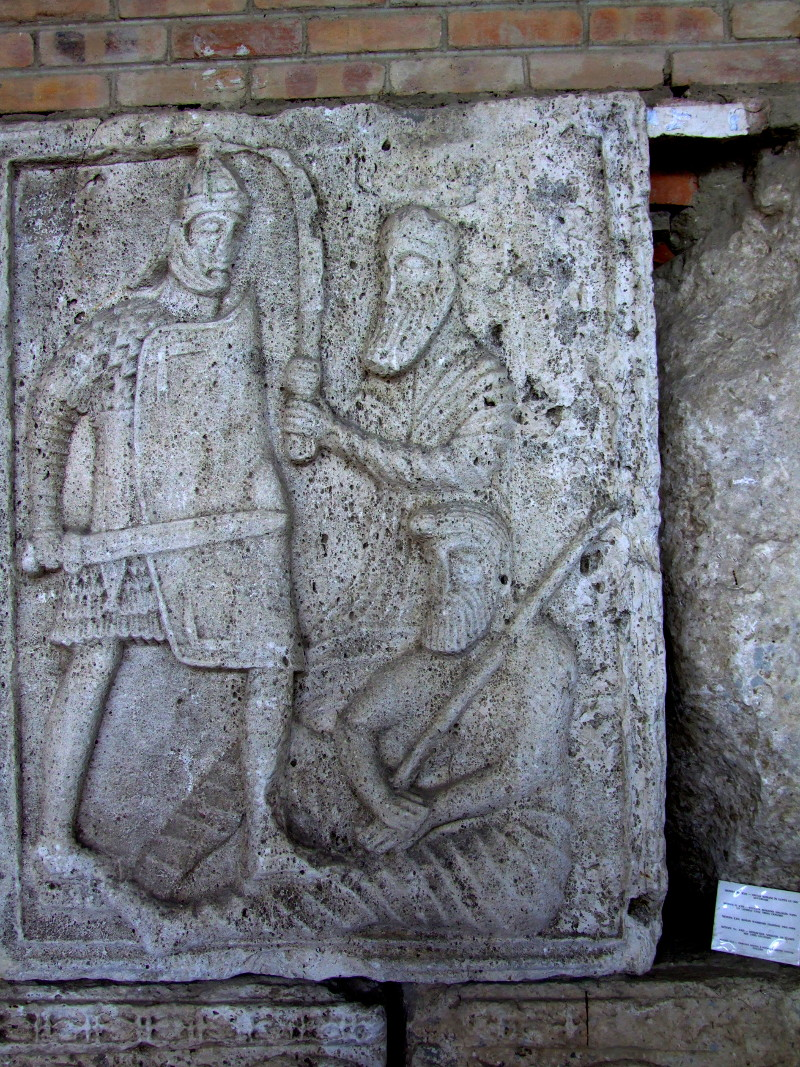
\includegraphics[width=0.75\textwidth]{../images/falx}~
\\[1cm]
\end{center}

Малък фалкс, сърп     & 5-12                 & 0.9м   & средни/високи (//-2)    & +2 на всички хвърляния срещу щитове   & 1.5кг   & евтин       \\
\begin{center}
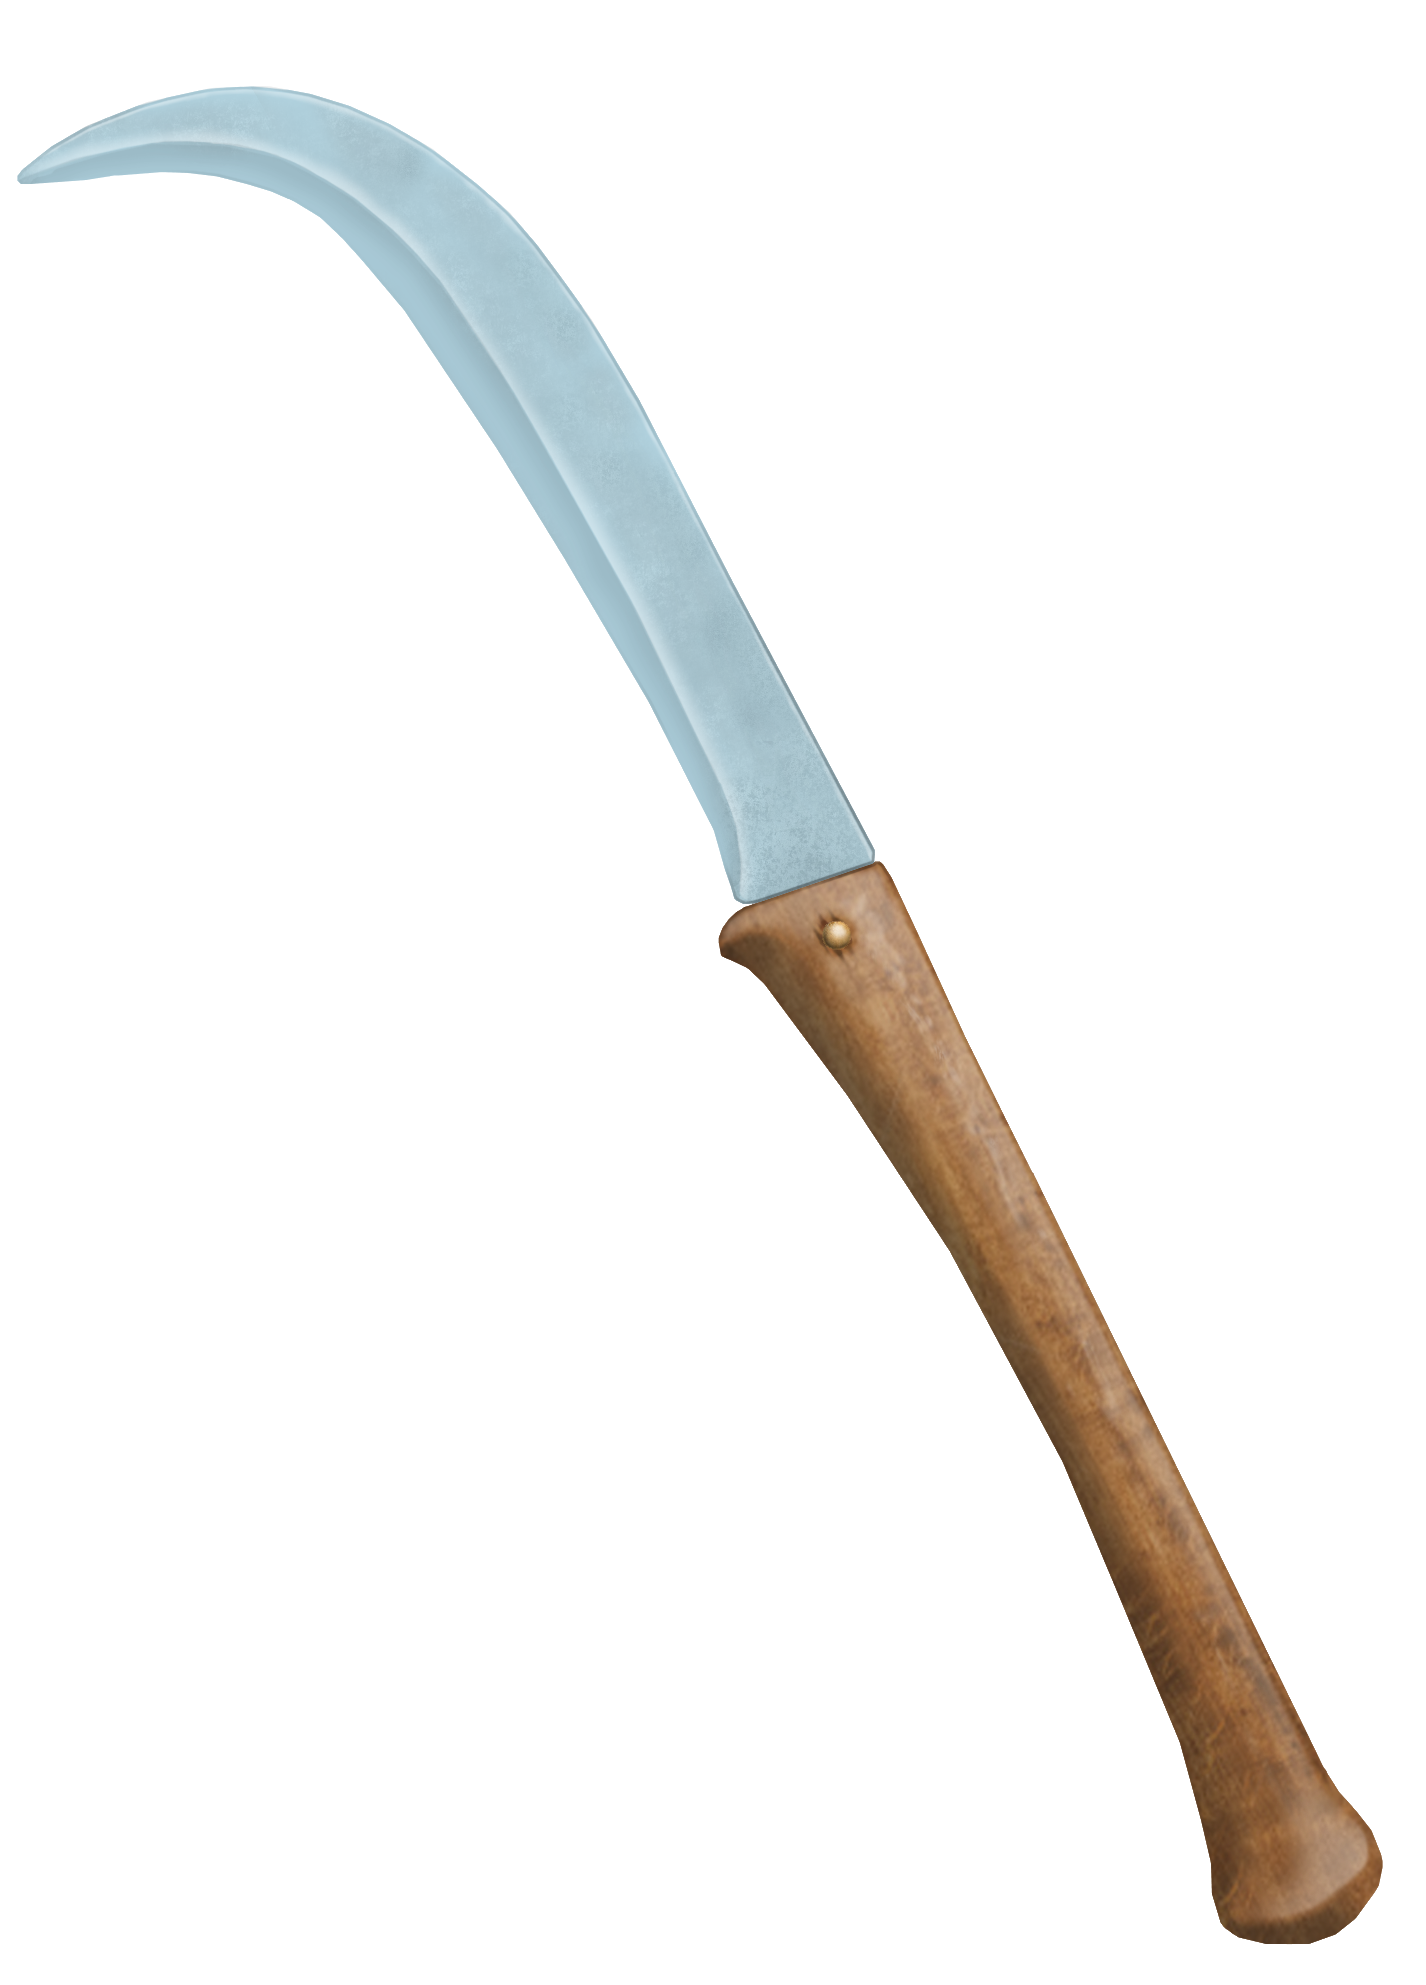
\includegraphics[width=0.75\textwidth]{../images/small_falx}~
\\[1cm]
\end{center}

Датска брадва         & 5-12                 & 1.2м & високи (+2/-2/-2) & бронебойност           & 1.5кг & евтин  \\
\begin{center}
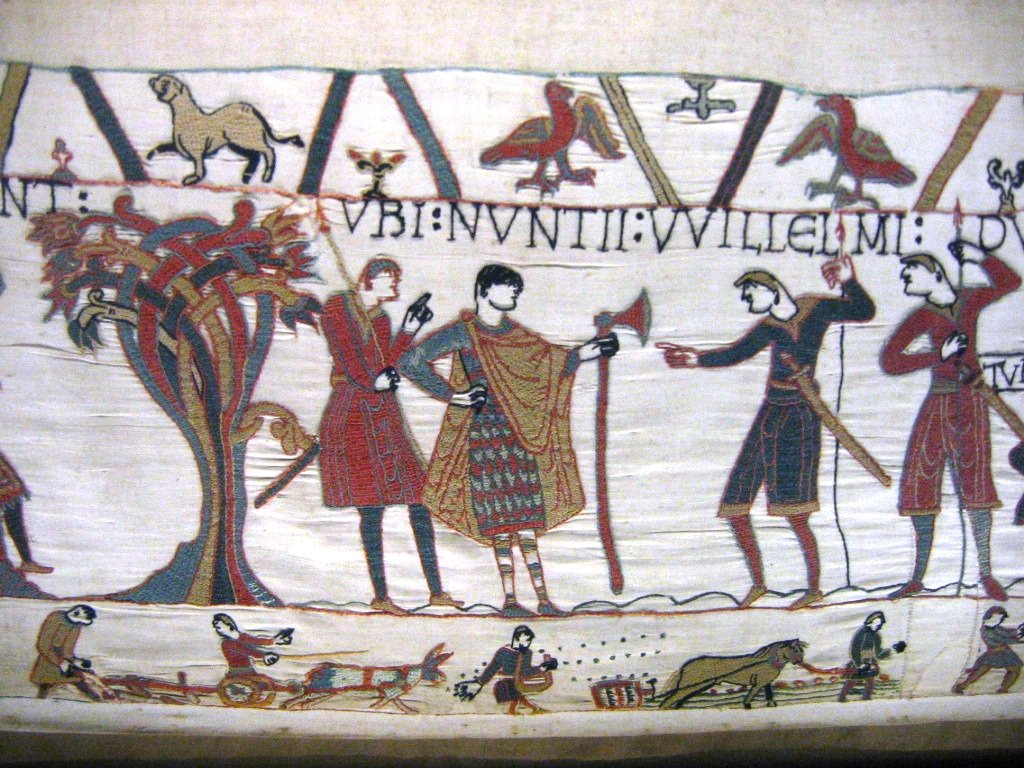
\includegraphics[width=0.75\textwidth]{../images/dane_axe}~
\\[1cm]
\end{center}

Алебарда             & 5-12                  & 1.7м      & високи (//-2)     & бронебойност, поваляне & 2.2кг & евтин  \\
\begin{center}
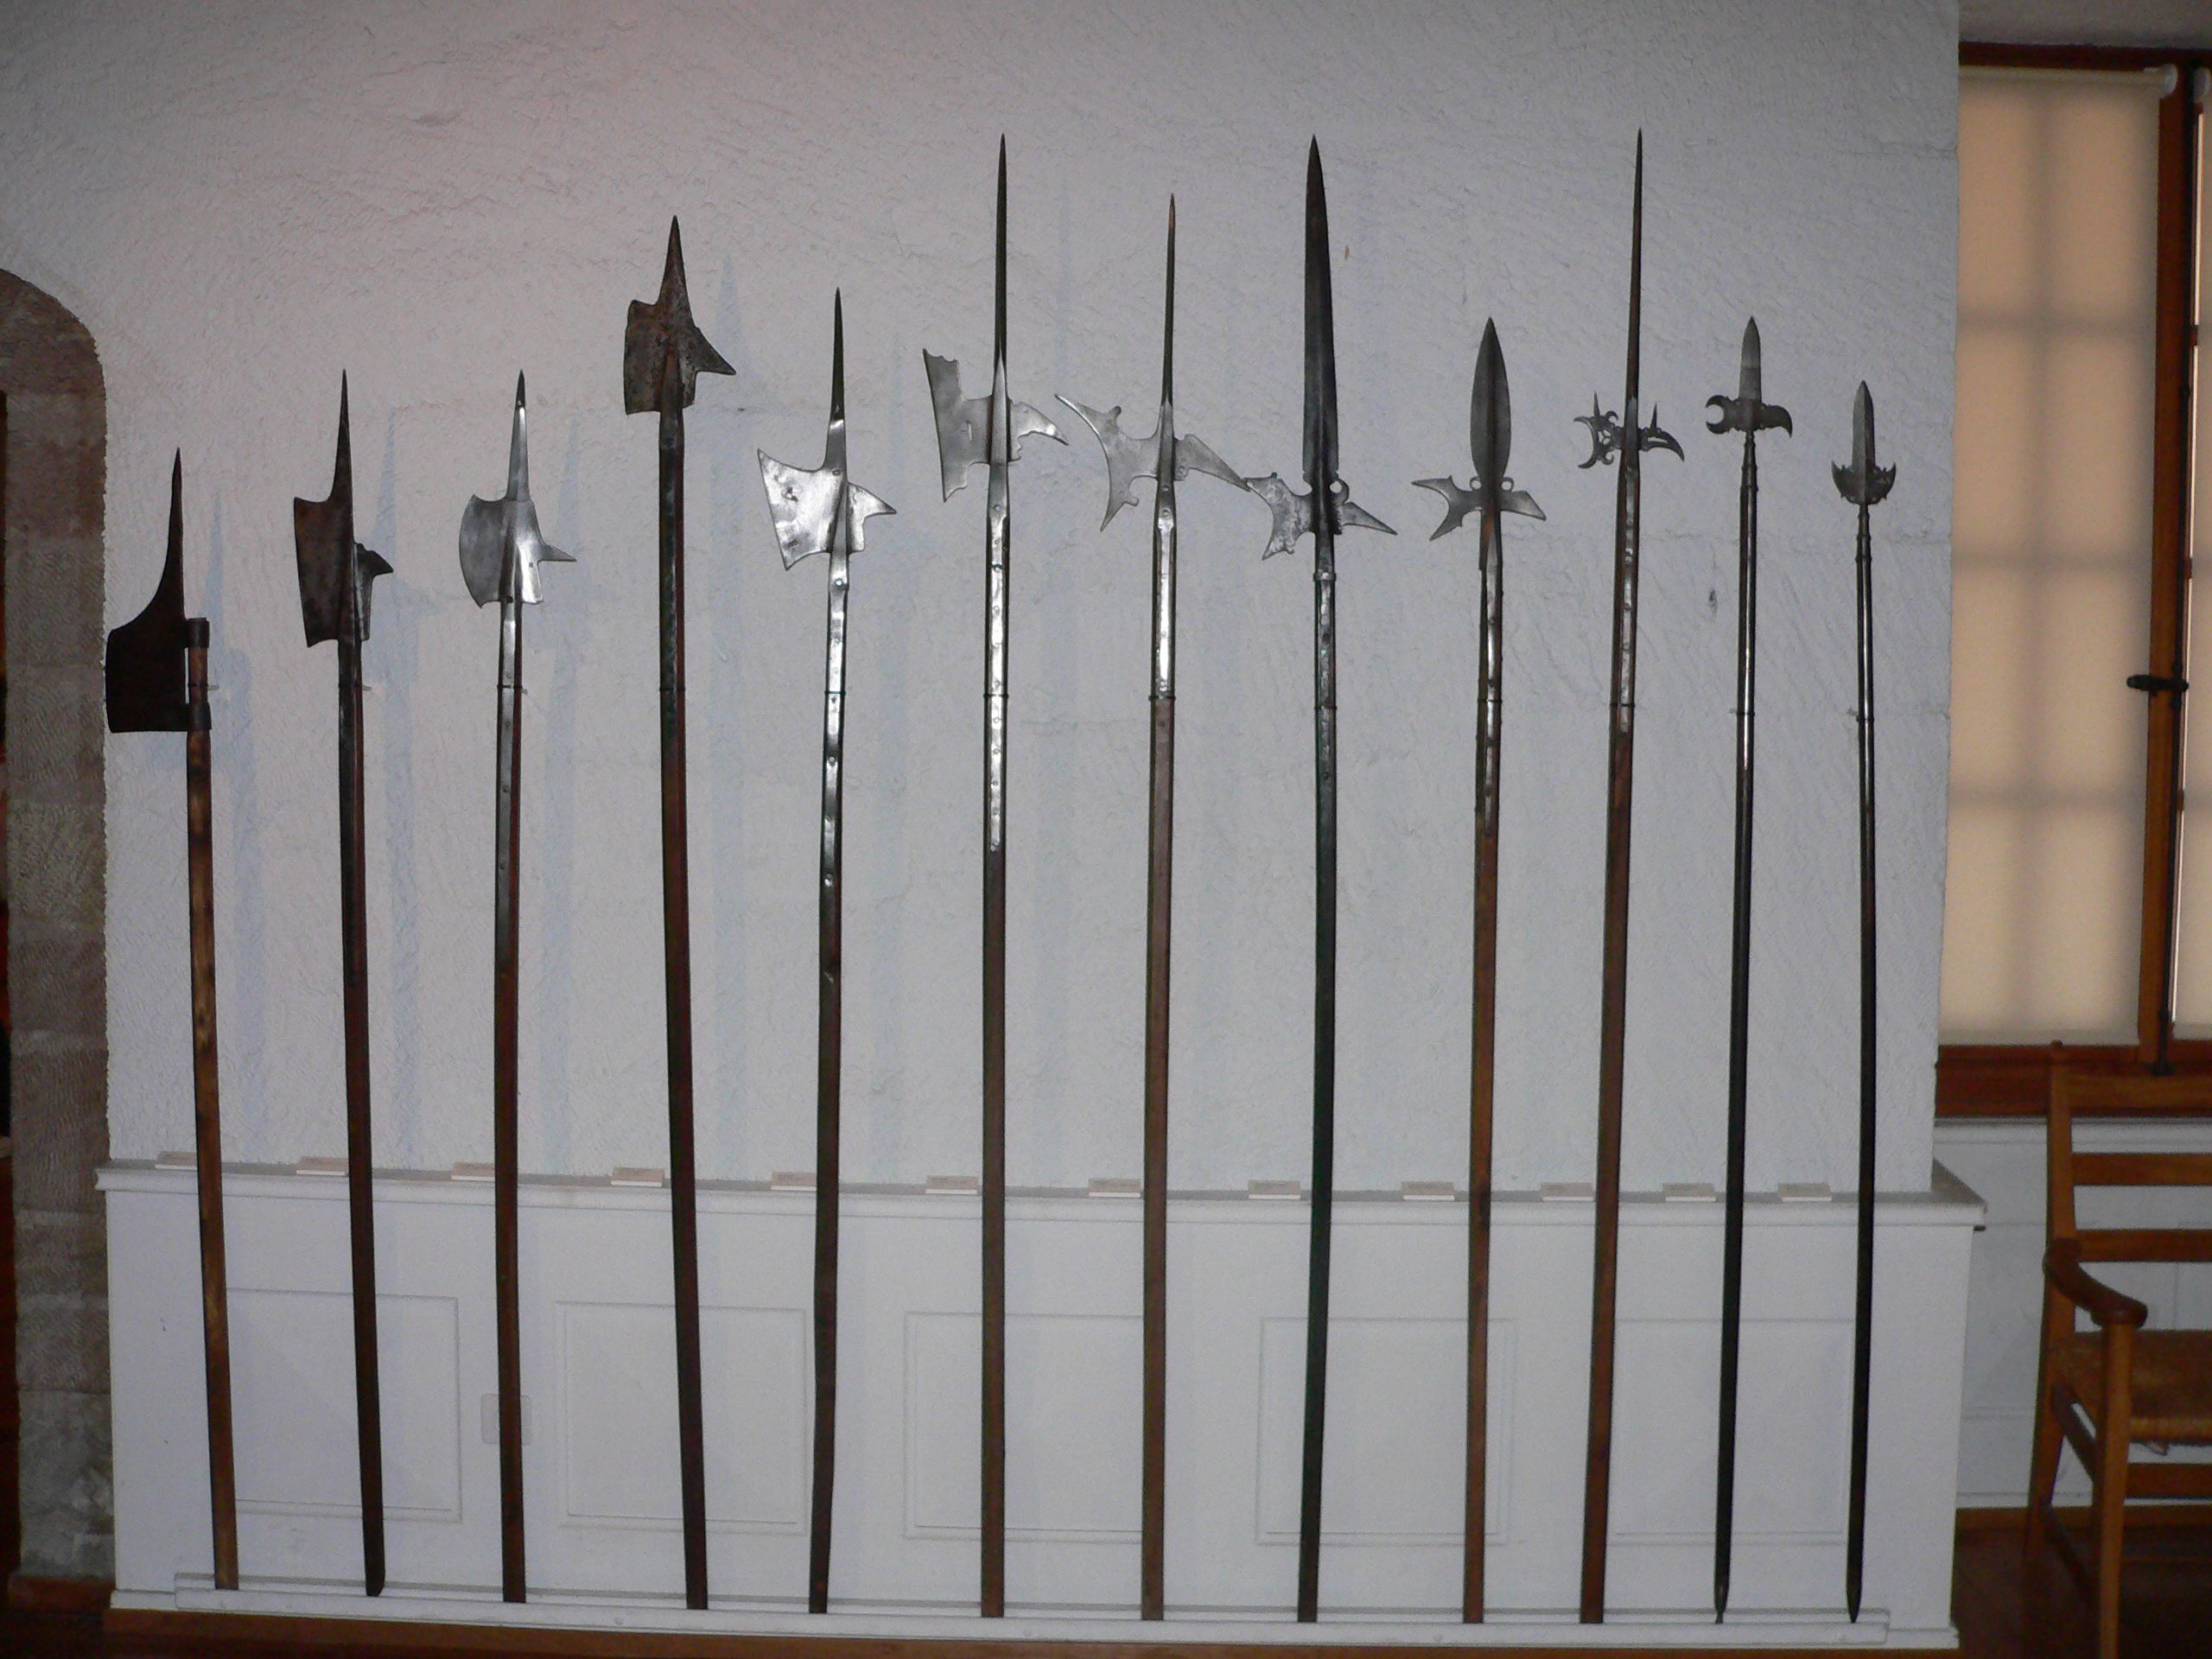
\includegraphics[width=0.75\textwidth]{../images/helbard}~
\\[1cm]
\end{center}

Пика                 & 5-12                 &  7м     & високи (//-2)    & повратливост   & 5кг   & евтин       \\
\begin{center}
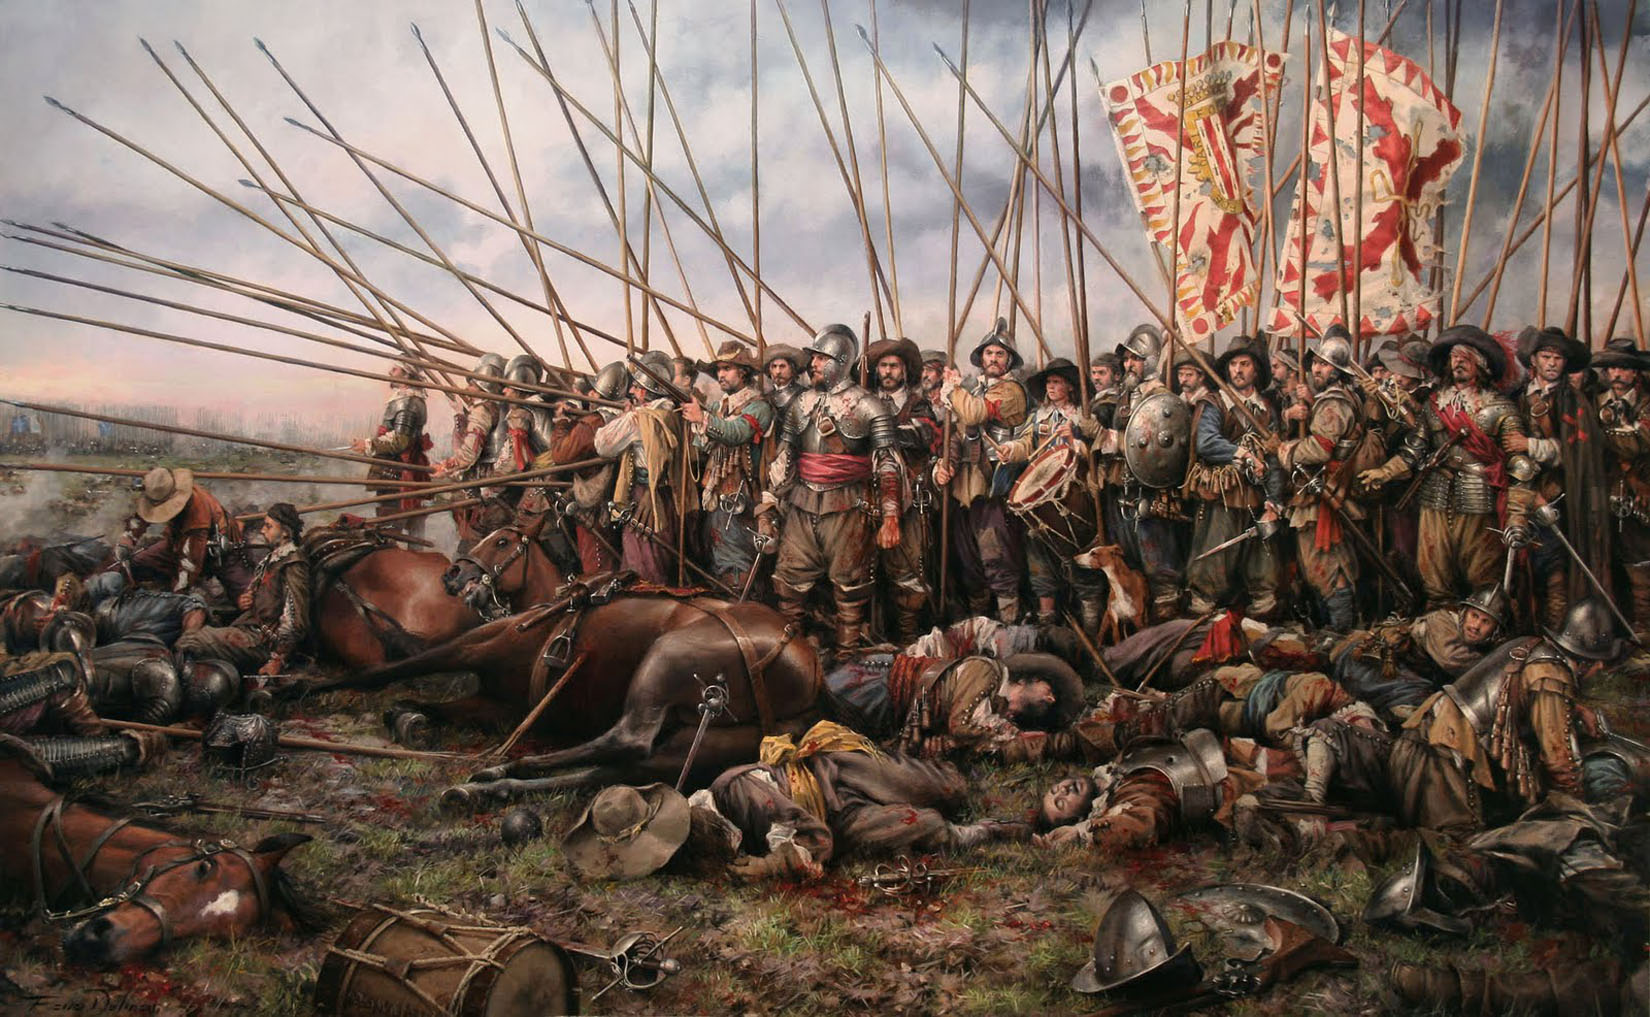
\includegraphics[width=0.75\textwidth]{../images/pike}~
\\[1cm]
\end{center}

Глейв, нагината      & 5-12                 & 2.5м & високи (+2/-2/-2) & бонус срещу щитове & 1.5кг & евтин  \\
\begin{center}
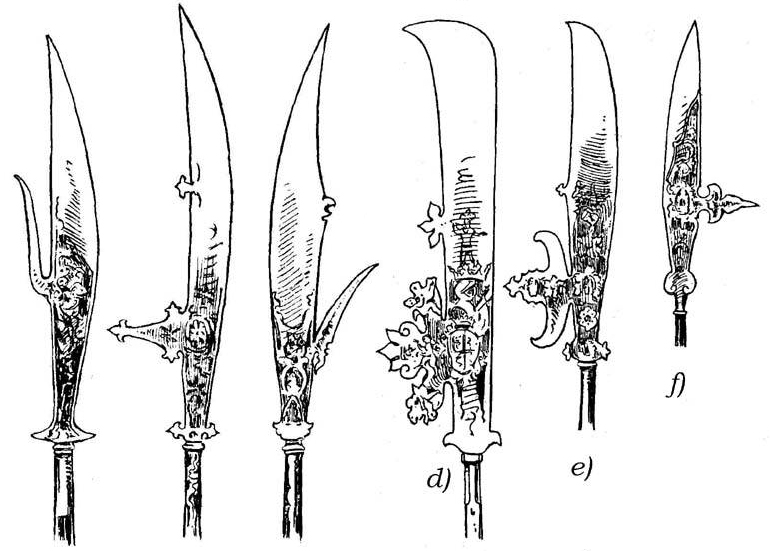
\includegraphics[width=0.75\textwidth]{../images/glavie}~
\\[1cm]
\end{center}
\begin{center}
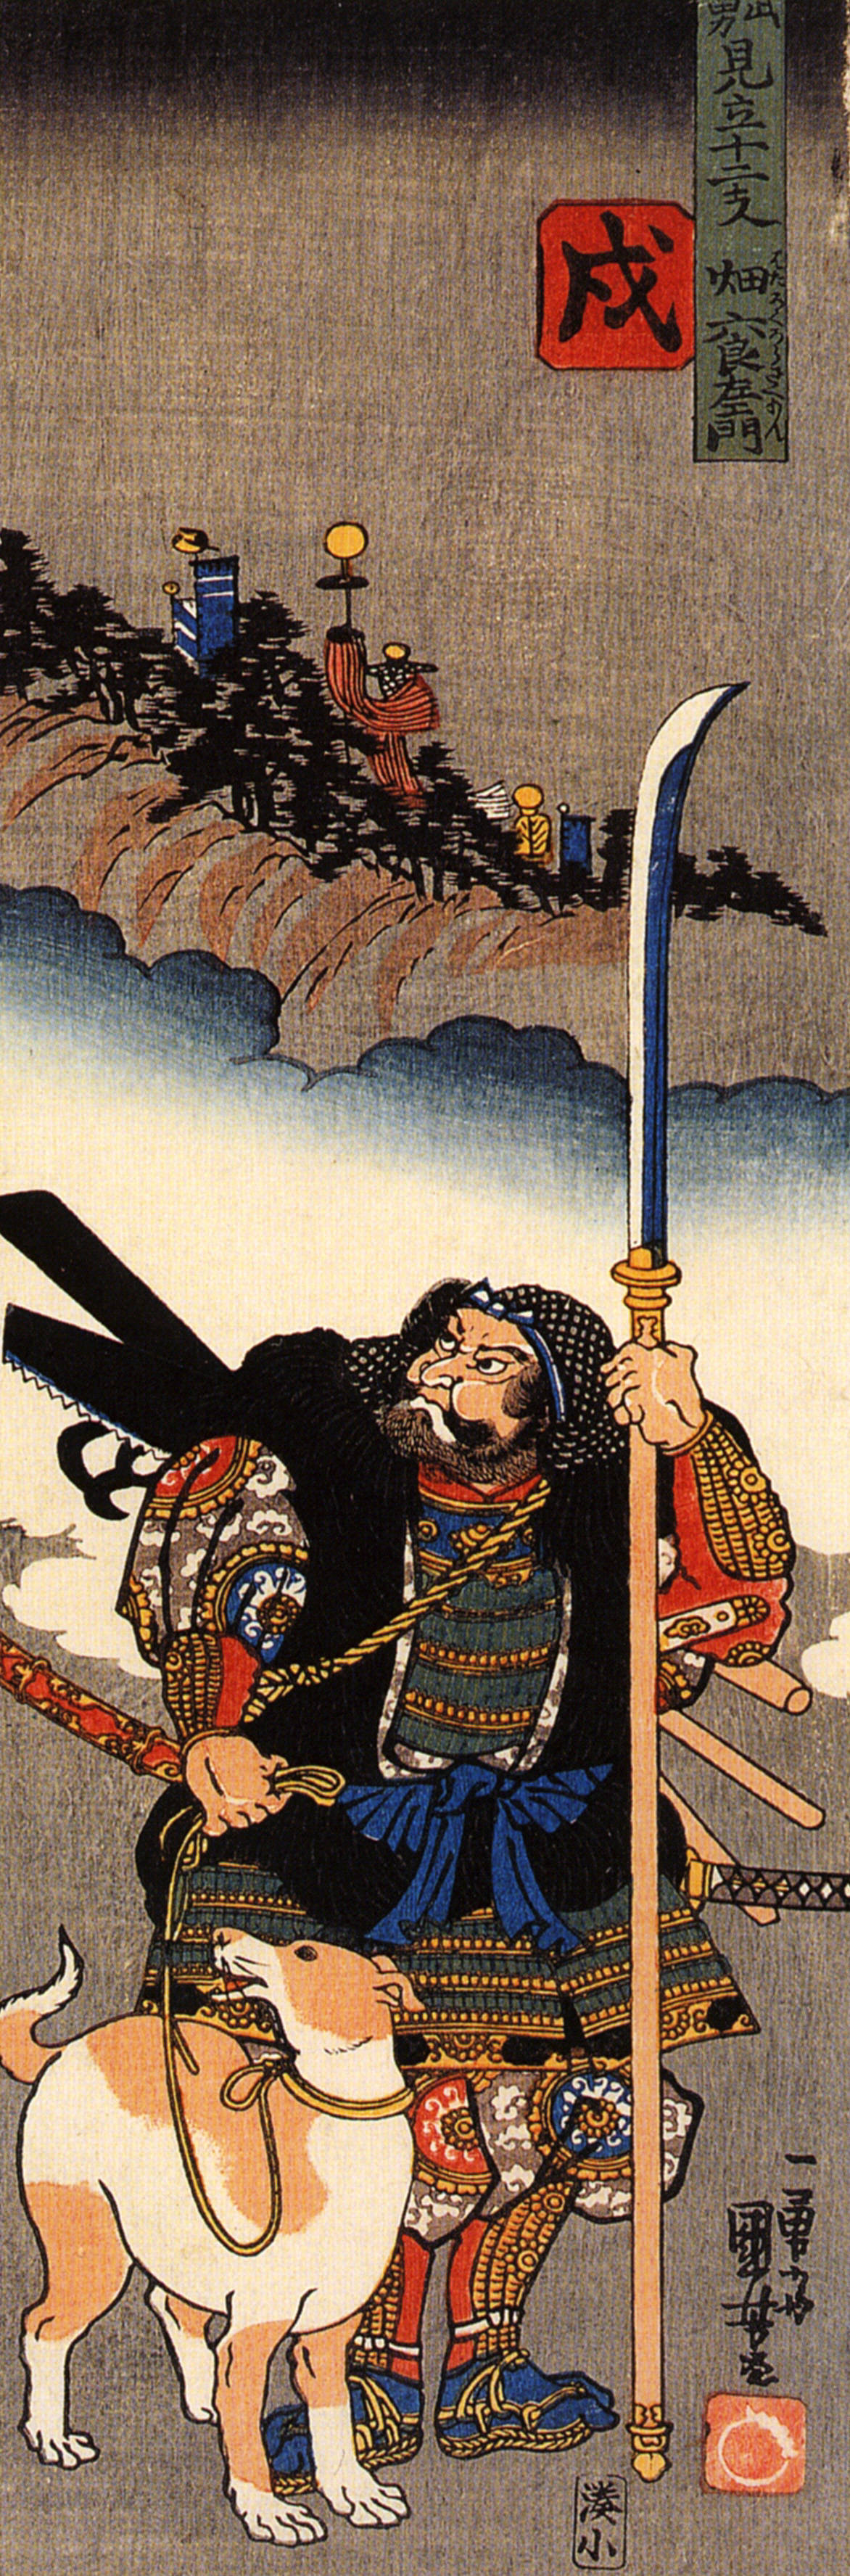
\includegraphics[width=0.75\textwidth]{../images/naginata}~
\\[1cm]
\end{center}

% Отдалечени атаки.
Метателен нож         & 3-9                  & (Сила/2)   & ниски      & -              & 0.2кг & много евтин  \\
Метателно копие       & 5-12                 & (Сила)     & средни     & -              & 1кг   & много евтин  \\
Дървен дълъг лък      & 7, зарежда се 1 ход  & (Сила х 2) & високи     & -              & 2кг   & евтин        \\
Малък арбалет         & 7, зарежда се 2 хода & (Сила х 2) & високи     & бронебойност I & 3кг   & евтин        \\
Арбалет               & 7, зарежда се 2 хода & (Сила х 2) & високи     & бронебойност I & 3кг   & евтин        \\
Арбалет с макара      & 5 необходима, 12 реална, зарежда се 10 хода & (Сила х 2) & високи & бронебойност II & 4кг & среден\\
Колчан 12 стрели      & -                    & -          & -          & -              & 1кг   & много евтин  \\

Бодкин стрела         & -                    & +3         & -3     & бронебойност       & 1.5кг & много евтин  \\
Широка стрела         & -                    & -          & -      &                    & 1.5кг & много евтин  \\
\begin{center}
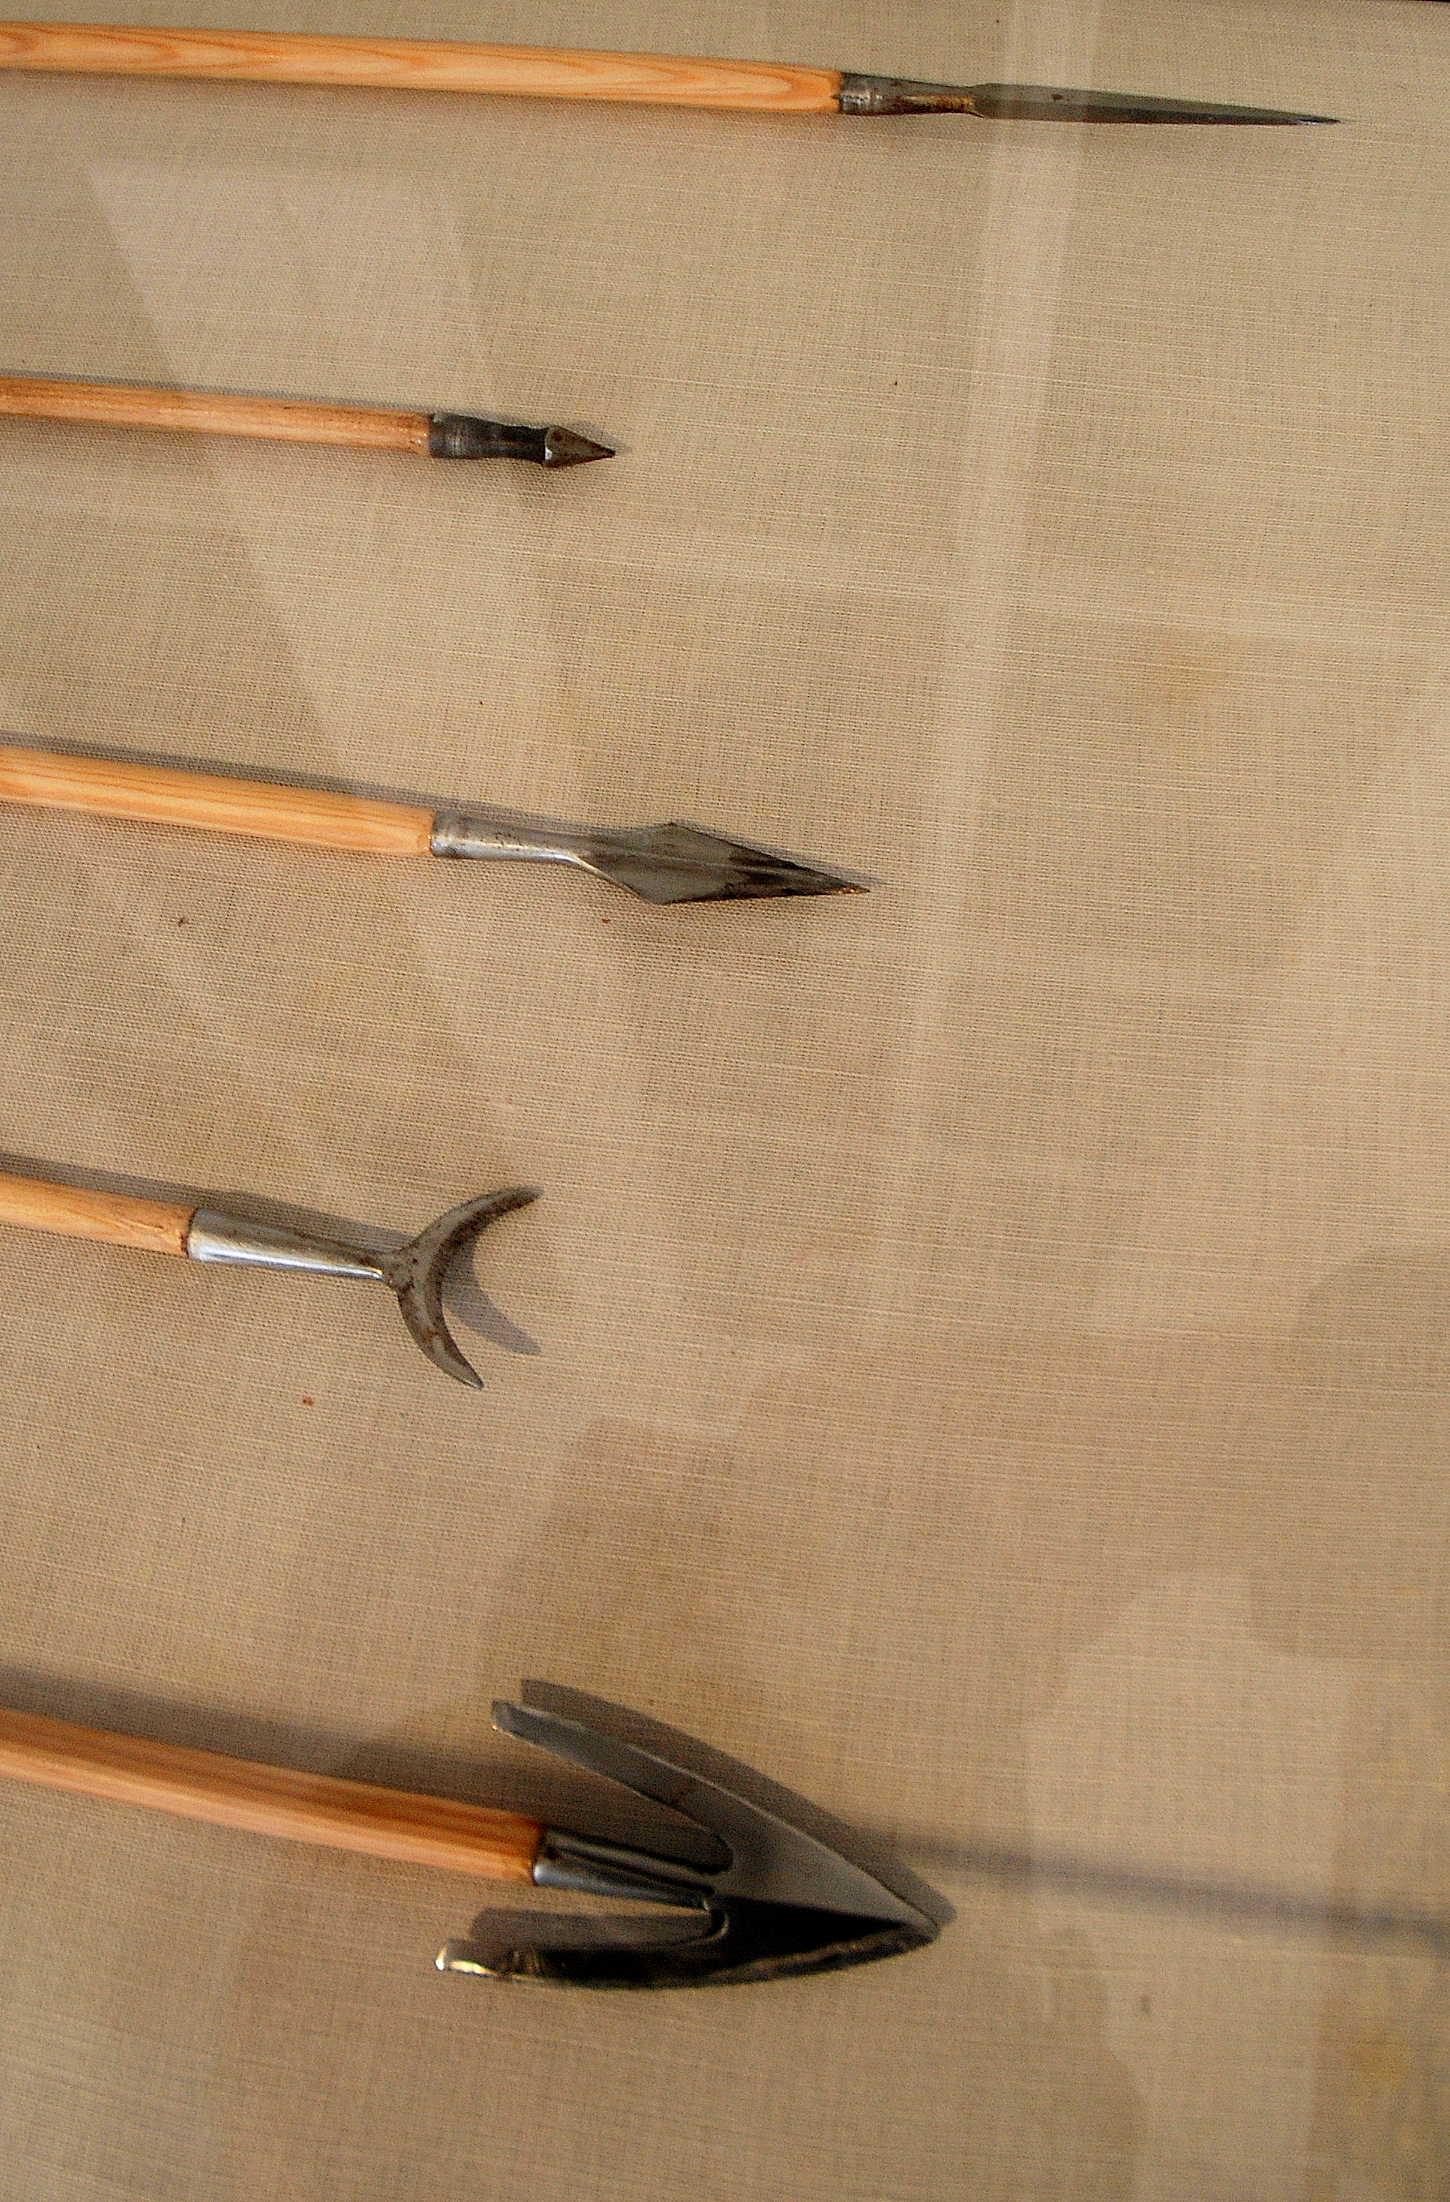
\includegraphics[width=0.75\textwidth]{../images/arrow}~
\\[1cm]
\end{center}

% Щитове.
Дървен щит 80см       & 5-12                 & близък     & ниски      & поваляне       & 2кг   & много евтин  \\
\end{tabular}

\subsection{Брони}
\textbf{Здравина}:
\begin{itemize}[topsep=-0cm, partopsep=0cm, parsep=0cm, itemsep=0cm]
\item{Кожена броня(слоеве памук/хартия/коприна/мека кожа, със зашити плочи варена кожа/хитинова коруба на негъвкавите части) 2}
\item{Халчеста броня, подплатена с гамбезон 4}
\item{Ламенарна броня, подплатена с гамбезон 6}
\item{Лята броня, подплатена с гамбезон(средновековен дизайн - субоптимална форма, субоптимална стомана, примитивно закаляване, подвижност в ставите се осигурява от халчести участъци) 8}
\item{Лята броня, подплатена с гамбезон(ренесансов дизайн - скосени повърхности, качествена стомана (high toughness core),  интелигентно закаляване на повърхностния слой(hardened shell), сложни механични стави) 10}
\\
\\
Масата на конпонент клони към една десета от произведенито на покритието и здравината му за средно качество изработка.
\end{itemize}

\subsection{Други}
комплект отрови - действие за някокко дена \\
алхимични принадлежности - кутия, хаван, стъкленици, лампа и т.н., 2кг, сренед  \\
стрела, клиновидна  \\
стрела, широка  \\


\section{Умения}
Означените със звездичка умения са събирателни понятия.
Например може да се избере \textit{елфически} език или оръжие \textit{брадва} или наука \textit{алхимия}.
\subsection{Общуване}
Лъжене (Чар)                      \\
Сплашване (Чар)                   \\
Изтезаване/Разпитване (Чар)       \\
Емпатия (Чар)                     \\
Четене по устните (Чар)           \\
Молене (Чар)                      \\

\subsection{Академични}
Език* (Ум)                        \\
Наука* (Ум)                       \\
Тактика (Ум)                      \\

\subsection{Схватки}
Оръжие* (Ловкост)                 \\
Военна машина* (Ум)               \\

\subsection{Придвижване}
Плуване (Сила)                    \\
Кaтерене (Сила)                   \\

\subsection{Занаяти}
Билкарсто (Ум)                    \\

\subsection{Епични провали}
Ако при мятане на д6* се падне -5 или +6, се мята отново.
Ако случайно се падне същото число, то се взема предивд и се продължава с мятането.
Ако крайният резултат е <0, имаме епичен провал, честито!  \\

При атака с оръжие           \\
- да го изтърве              \\
- да се сепъне               \\
- да се наръга               \\
- да се счупи                \\
- да удари някого другиго    \\
- ми нищо не се случва       \\

\chapter{Качества}

\textbf{Положителни}
\begin{itemize*}
\item{Виждане в тъмнина}
\item{Съюзник - съюзник, влиятелна личност или организация, което дължи услуги на персоанжа}
\item{Нестареещ - не заплашван от старост иили изтичане на дните}
\item{Заможен - започваш допълнително с един скъп предмет}
\item{Общуване с животни}
\item{Кристален слух}
\end{itemize*}

\vspace{0.7cm}
\textbf{Отрицателни}
\begin{itemize*}
\item{куцане (1/4 скорост)}
\item{слаб слух}
\item{нелогичен панически страх от паяци/змии/широки отркити пространства/тесни затворени пространства/височини}
\item{късогледство/далекогледство}
\item{нелогично неустоимо приличане към огън/силно психоактивно вещество/сексъално към деца/изричане на лъжи/физически конфликт}
\item{обезобразено лице}
\item{малодушие}
\item{заблуда (A dellusion is a fixed belief that is either false, fanciful, or derived form deception, held despite evidence to the contrary.)}
\item{тревожност (параноя)}
\item{мързел (безинициативност)}
\item{асоциалност}
\item{крайно скъперничество}
\item{крайна срамежливост}
\item{крайна самоувереност}
\item{краен песимизъм}
\item{наднормено тегло}
\item{Враг - индивид или организация, готови да отделят ресутрси само за да навредят на персонажа}
\item{Беден - започваш само с дрехи}
\item{Кръвожадност}
\item{Късогледство/Далекогледство - -10 наблюдателност и боравене на далеч/близо}
\end{itemize*}


\tableofcontents
\end{document}
